%package list
\documentclass{article}
\usepackage[top=3cm, bottom=3cm, outer=3cm, inner=3cm]{geometry}
\usepackage{graphicx}
\usepackage{url}
%\usepackage{cite}
\usepackage{hyperref}
\usepackage{array}
%\usepackage{multicol}
\newcolumntype{x}[1]{>{\centering\arraybackslash\hspace{0pt}}p{#1}}
\usepackage{natbib}
\usepackage{pdfpages}
\usepackage{multirow}
\usepackage{multirow}
\usepackage[normalem]{ulem}
\useunder{\uline}{\ul}{}
\usepackage{amsmath}
\usepackage{float}
\usepackage{multicol}
\usepackage{subcaption}
%%%%%%%%%%%%%%%%%%%%%%%%%%%%%%%%%%%%%%%%%%%%%%%%%%%%%%%%%%%%%%%%%%%%%%%%%%%%
%%%%%%%%%%%%%%%%%%%%%%%%%%%%%%%%%%%%%%%%%%%%%%%%%%%%%%%%%%%%%%%%%%%%%%%%%%%%
\newcommand{\csemail}{vmachacaa@ulasalle.edu.pe}
\newcommand{\csdocente}{MSc. Vicente Enrique Machaca Arceda}
\newcommand{\cscurso}{Tópicos en Computación Gráfica}
\newcommand{\csuniversidad}{Universidad San Agustín de Arequipa}
\newcommand{\csescuela}{Doctorado en Ciencias de la Computación}
\newcommand{\cspracnr}{03}
\newcommand{\cstema}{Predicción y modelado en 3D de estructuras terciarias de proteinas a partir del \textit{contact map}}
%%%%%%%%%%%%%%%%%%%%%%%%%%%%%%%%%%%%%%%%%%%%%%%%%%%%%%%%%%%%%%%%%%%%%%%%%%%%
%%%%%%%%%%%%%%%%%%%%%%%%%%%%%%%%%%%%%%%%%%%%%%%%%%%%%%%%%%%%%%%%%%%%%%%%%%%%


\usepackage[english,spanish]{babel}
\usepackage[utf8]{inputenc}
\AtBeginDocument{\selectlanguage{spanish}}
\renewcommand{\figurename}{Figura}
\renewcommand{\refname}{Referencias}
\renewcommand{\tablename}{Tabla} %esto no funciona cuando se usa babel
\AtBeginDocument{%
	\renewcommand\tablename{Tabla}
}

\usepackage{fancyhdr}
\pagestyle{fancy}
\fancyhf{}
\setlength{\headheight}{30pt}
\renewcommand{\headrulewidth}{1pt}
\renewcommand{\footrulewidth}{1pt}
\fancyhead[L]{\raisebox{-0.2\height}{
\includegraphics[width=3cm]{img/logo_unsa}}}
\fancyhead[C]{}
\fancyhead[R]{\fontsize{7}{7}\selectfont	\csuniversidad \\ \csescuela \\ \textbf{\cscurso} }
\fancyfoot[L]{MSc. Vicente Machaca}
\fancyfoot[C]{\cscurso}
\fancyfoot[R]{Página \thepage}


% para el codigo fuente
\usepackage{listings}
\usepackage{color}
\definecolor{dkgreen}{rgb}{0,0.6,0}
\definecolor{gray}{rgb}{0.5,0.5,0.5}
\definecolor{mauve}{rgb}{0.58,0,0.82}
\lstset{frame=tb,
	language=Python,
	aboveskip=3mm,
	belowskip=3mm,
	showstringspaces=false,
	columns=flexible,
	basicstyle={\small\ttfamily},
	numbers=none,
	numberstyle=\tiny\color{gray},
	keywordstyle=\color{blue},
	commentstyle=\color{dkgreen},
	stringstyle=\color{mauve},
	breaklines=true,
	breakatwhitespace=true,
	tabsize=3
}




\begin{document}
	
	\vspace*{10px}
	
	\begin{center}	
		\fontsize{17}{17} \textbf{ ArgosMol: Una plataforma web para la visualización de estructuras de proteinas }
	\end{center}
	%\centerline{\textbf{\underline{\Large Título: Informe de revisión del estado del arte}}}
	%\vspace*{0.5cm^
	

	\begin{table}[h]
		\begin{tabular}{|x{4cm}|x{6.3cm}|x{4cm}|}
			\hline 
			\textbf{ALUMNO} & \textbf{PROGRAMA}  & \textbf{CURSO}   \\
			\hline 
			\csdocente & \csescuela & \cscurso    \\
			\hline 
		\end{tabular}
	\end{table}	
	
		
	
\section{Introducción}
	
	Las proteínas son moléculas complejas que cumplen un rol crítico en nuestro cuerpo, estas cumplen la mayoria de funciones en la células \citep{anderson1998proteome}. Además, la función de una proteína depende de su estructura \citep{rangwala2010introduction} y recientemente se ha descubierto que esta función tambien depende de las relación de una proteina con otras \citep{canzarprotein}. Mas aún, es importante saber, que la estructura de una proteina puede cambiar en el tiempo y su función tambien cambia en el tiempo. Conocer la estructura de una proteína es de suma importancia para el análisis de su función, generación de medicamentos, etc. \citep{rangwala2010introduction}. Además, lograr predecir y entender el funcionamiento de estas proteinas y la interacción de redes de proteínas es considerado el nuevo santo crial de la Binformática en estos tiempos \citep{srihari2017computational}. \\
	

	Adicionalmente, una de las tares mas  utilizadas en Bioinformática es la visualización de moleculas \citep{o2010visualization, mura2010introduction}. La visualización de los \textit{Ligand-binding} y detalles de las macromoleculas ayudan a comprender la relación de una estructura de proteína con su función \citep{reynolds2018ezmol}. Además, en la actualidad la visualización de estructuras de proteína pueden ser realizados a traves de herramientas Web, dejando de lado otras herramientas que requieren instalación \citep{wang2020icn3d}. Esto ha acasionado, que se empiece el desarrollo de herramientas Web para la visualización de proteínas, pero estas son pocas, tienen errores y algunas no son intuitivas y dificiles de utilizar.\\
	
		
	Frente a la problematica mencionada anteriormente, se propone la herramienta Web ArgosMol, esta plataforma tiene el objetivo de ser facil de usar, seguir los principios propuestos por \cite{youkharibache2017twelve} y mantener una relación constante entre el modelo 3D y la secuencia de aminoacidos (cualquier acción realizada en el modelo, se refleja en la secuencia de aminoacidos y viceversa). 	
	
	
\section{Marco teórico}
	
	En esta sección detallaremos algunos conceptos previos del area de Bioinformática/\textit{Proteomics} para comprender el trabajo.
	
	
	\subsection{Aminoacidos}
		
	Deacuerdo a \cite{medlineplus_2021}, los aminoácidos son compuestos orgánicos que se combinan entre ellos para formar proteínas. En otras palabras, las proteínas estan hechas de aminoacidos. Tenemos tres tipos de aminoacidos: 
	
	\begin{itemize}
		\item \textbf{Esenciales}: El cuerpo no los puede producir, entonces debemos consumirlos en los alimentos. Los 9 aminoácidos esenciales son: histidina, isoleucina, leucina, lisina, metionina, fenilalanina, treonina, triptófano y valina.
		\item \textbf{No esenciales}: El cuerpo es capaz de producir estos aminoacidos y estos son: alanina, arginina, asparagina, ácido aspártico, cisteína, ácido glutámico, glutamina, glicina, prolina, serina y tirosina.
		\item \textbf{Condicionales}: Por lo regular no son esenciales, excepto en momentos de enfermedad y estrés, los aminoacidos condicionales son: arginina, cisteína, glutamina, tirosina, glicina, ornitina, prolina y serina. 
	\end{itemize}
	
	\subsection{Estructura de las proteinas}
	
	Existen 4 tipos de estructuras de proteínas \citep{russell2002igenetics}:
	
	\begin{enumerate}
		\item \textbf{Estructura primaría:} Secuencia de aminoacidos (ver Figura \ref{fig:protein_structure} (a)).
		\item \textbf{Estructura secundaría:} Pequeños patrones, los mas comunes son las elises $\alpha$ y hojas $\beta$ (ver Figura \ref{fig:protein_structure} (b)).
		\item \textbf{Estructura terciaría:} Representa la unión de los segmentos de la estructura secundaría (ver Figura \ref{fig:protein_structure} (c)). En este caso solo estamos considerando una cadena de aminoacidos (las proteinas a veces son conformadas por varias cadenas de aminoacidos).
		\item \textbf{Estructura cuaternaría:} Union de varias estructuras terciarias (varias cadenas de aminoacidos) (ver Figura \ref{fig:protein_structure} (d)).
	\end{enumerate}
	
	
	\begin{figure}[H]
		\centering
		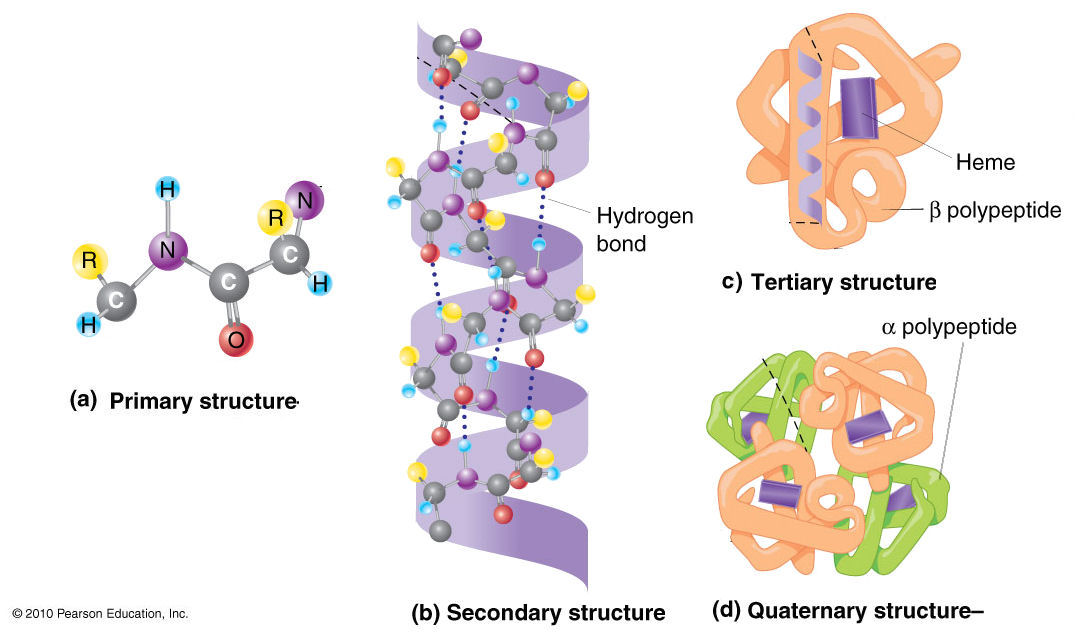
\includegraphics[width=0.6\textwidth]{img/papers/protein_structure}
		\caption{Ejemplo de las 4 estructuras de proteínas. Fuente: \citep{russell2002igenetics}}
		\label{fig:protein_structure}
	\end{figure}
	
	
	\subsection{\textit{Contact map}}
	
	Representa la distancia de cada posible aminoacido, cuando forman proteínas. El \textit{contact map}, es representado como un gráfico en 2D, y es el elegido por los modelos de machine learning en la predicción de las estructuras de proteínas. En la Figura \ref{fig:contact_map}, mostramos como es un \textit{contact map}.
	
	\begin{figure}[H]
		\centering
		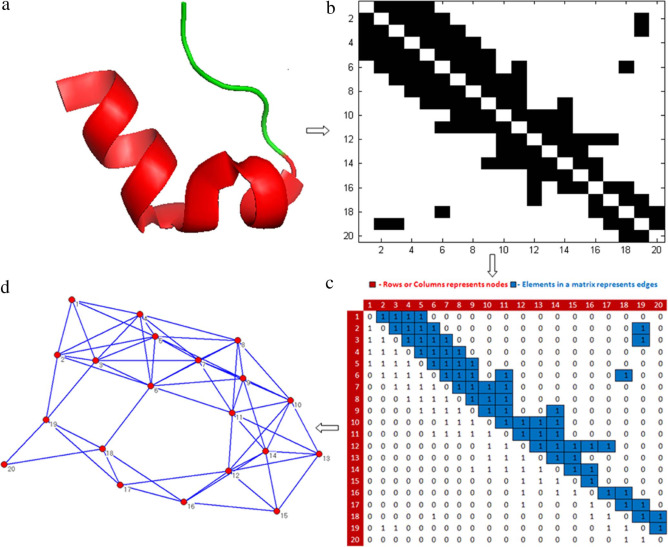
\includegraphics[width=0.4\textwidth]{img/papers/contact_map}
		\caption{Ejemplo del contact map de una proteína.}
		\label{fig:contact_map}
	\end{figure}
	
	
	
	
\section{Trabajos relacionados}

Las herramientas mas utilizadas para la visualización de proteínas son herramientas de escritorio, entre estás tenemos: Chimera \citep{pettersen2004ucsf}, PyMol \citep{pymol2017pymol} y CnD3 \citep{wang2000cn3d}. Una de las principales desventajas de estas aplicaciones es que no son faciles de utilizar y requieren ser instaladas. Debido a esta problematica, en los ultimos años se ha empezado el desarrollo de herramientas Web que permiten visualizar proteínas con el menor esfuerzo posible. \\

Una de las primeras propuestas es \href{http://jolecule.com/}{Jolecule}, esta herramienta es desarrollada por Bosco Ho desde el 2011, aunque no tiene una publicación, es una herramienta con constante desarrollo hasta la actualidad. Dicha aplicación esta desarrollada sobre three.js y es de código libre. Jolecule, tiene algunos problemas de renderización, por momentos ciertas partes de la proteína no se visualizan. Tambien, en su página no se permite cargar una archivo .pdb para visualizarlo al menos que levatemos la aplicación en nuestro servidor. \\

La herramienta \href{https://nglviewer.org/}{NGL}  propuesta por \cite{rose2015ngl}, tambien está desarrollada sobre three.js y es de código libre. Aunque, en ciertas ocaciones la aplicación presenta errores, es una aplicación facil de utilizar.\\

Quizas, la herramienta mas intuitiva y con mayor cantidad de esquemas de colores y formas de visualización es \href{http://web3dmol.net/}{Web3DMol}. Propuesta por \cite{shi2017web3dmol}, esta herramienta permite permite ver a una sola vista el modelo 3D y la secuencia de aminoacidos (ambos completamente relacionados).\\

\href{http://www.sbg.bio.ic.ac.uk/ezmol/}{EzMol} propuesta por \cite{reynolds2018ezmol} es una aplicación  desarrollada sobre 3dmol.js. Según los autores, el objetivo de EzMol, es ser  una herramietna de facil uso. EzMol, tiene un \textit{wizard} que guia al usuario durante el proceso de visualización, este \textit{wizard} es util para usuarios inexpertos pero le resta puntos de usabilidad a la aplicación.  \\


Finalmente tenemos \href{https://www.ncbi.nlm.nih.gov/Structure/icn3d/full.html}{iCn3D}, propuesta por  \cite{wang2020icn3d}. Esta herramienta tambien ha sido desarrollada sobre three.js. Esta aplicación, tiene mas funcionalidades que las otras herramientas mencionadas anteriormente y tambien es de facil uso. Lamentablemente la herramienta no permite ver la secuencia de aminoacidos en forma paralela al modelo 3D y tambien tiene algunos problemas  con la posición de sus menus y botones.




\section{Propuesta}
	
ArgosMol surge como una alternativa a  herramientas \textit{desktop} como: Chimera \citep{pettersen2004ucsf}, PyMol \citep{pymol2017pymol} o CnD3 \citep{wang2000cn3d}, considerando que en estos ultimos años, se ha priorizado el desarrollo de herramientas Web que hacen uso de WebGL \footnote{Librería para el desarrollo de modelos 3D. \href{https://get.webgl.org/}{Enlace.}}, 		
Three.js \footnote{Librería de alto nivel para el desarrollo de modelos 3D, hace uso de WebGL. \href{https://threejs.org/}{Enlace.}} y 		
3DMol.js. \footnote{Librería para el modelado de átomos y moleculas, hace uso de WebGL. \href{https://threejs.org/}{Enlace.}}; Además, ArgosMol ha tomado en cuenta los principios de desarrollo de toda aplicación de visualización de moleculas, presentado por \cite{youkharibache2017twelve} \\

Para el desarrollo de ArgosMol se ha utilizado 3dmol.js y p5.js en el \textit{frontend} y PHP en el \textit{backend}. La herramienta es presentada en la Figura \ref{fig:argos1} y esta disponible en este \href{http://134.209.44.160/argosmol/protein_interaction.php}{enlace}. \\

\begin{figure}[H]
	\centering
	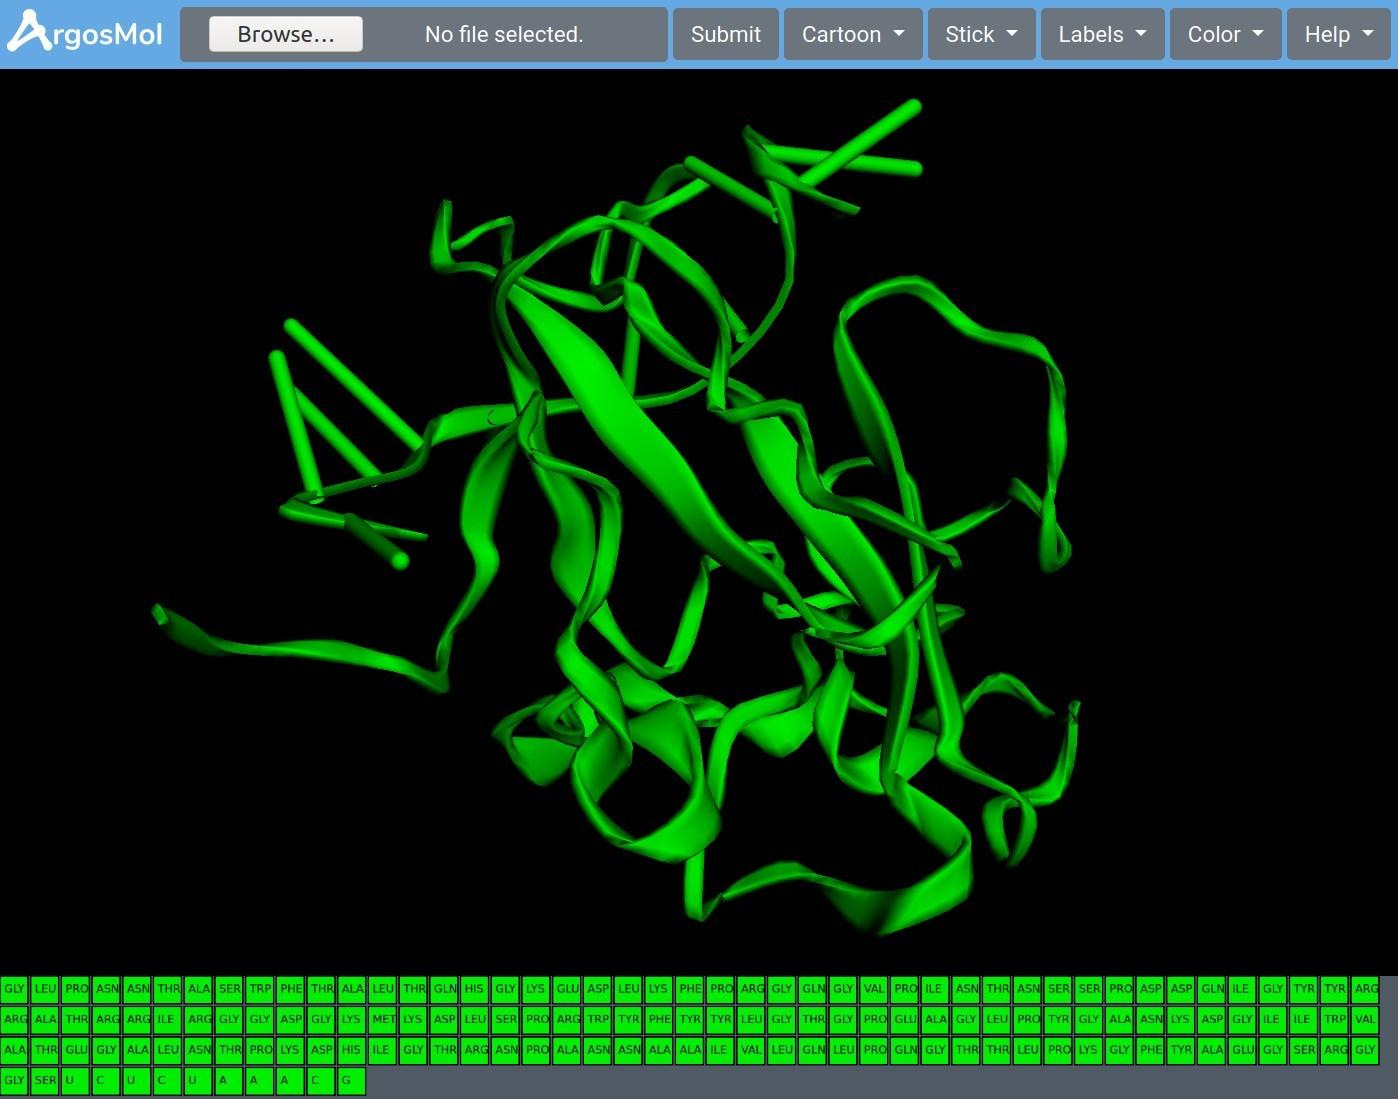
\includegraphics[width=\textwidth]{img/argosmol/mol1}
	\caption{ Ejemplo de visualización de proteínas con ArgosMol. }
	\label{fig:argos1}
\end{figure}



\subsection{Estilo}

ArgosMol permite ver la estructura de una proteína en tres modos distintos: \textit{Cartoon}, \textit{Stick} y \textit{Trace}, y la combinación de estos. Por ejemplo para la proteína con el identificador: \textit{7act} en el \textit{Protein Data Bank}. En la Figura \ref{fig:cartoon}, mostramos las 3 formas de visualización de ArgosMol, la Figura \ref{fig:cartoon}(a)(b)(c)(d) representan la proteína en un estilo \textit{cartoon}, \textit{trace}, \textit{stick}, \textit{cartoon}/\textit{stick} respectivamente. \\

\begin{figure}[H]
	\begin{subfigure}{.5\textwidth}
		\centering
		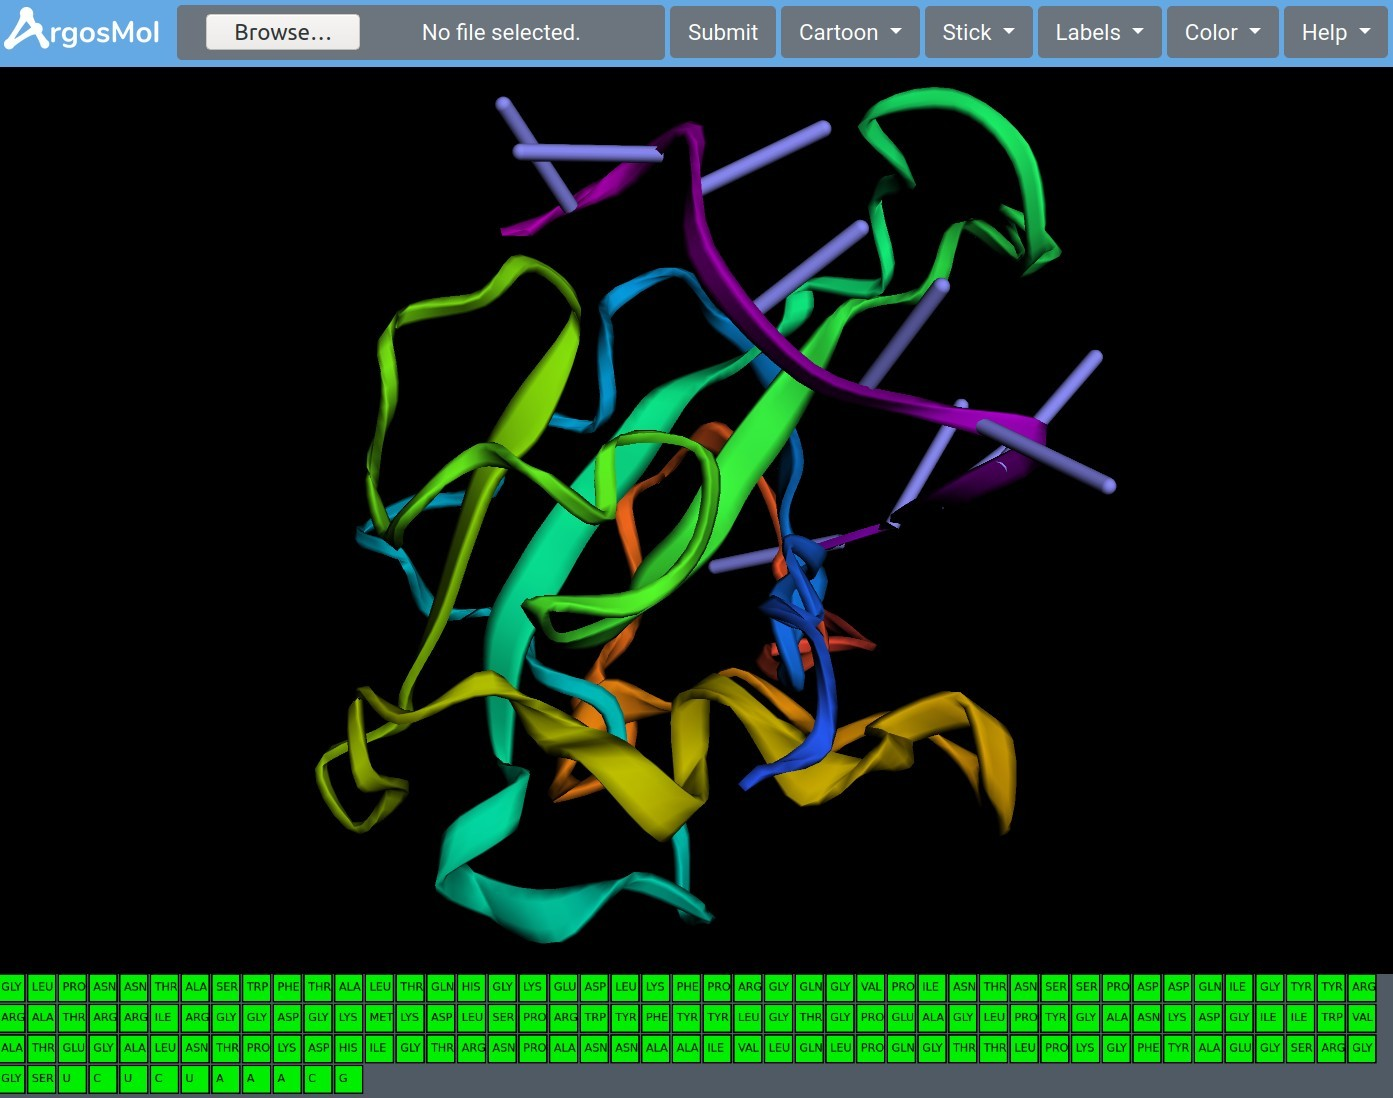
\includegraphics[width=.99\linewidth]{img/argosmol/mol2}
		\caption{}
		\label{fig:sfig1}
	\end{subfigure}%
	\begin{subfigure}{.5\textwidth}
		\centering
		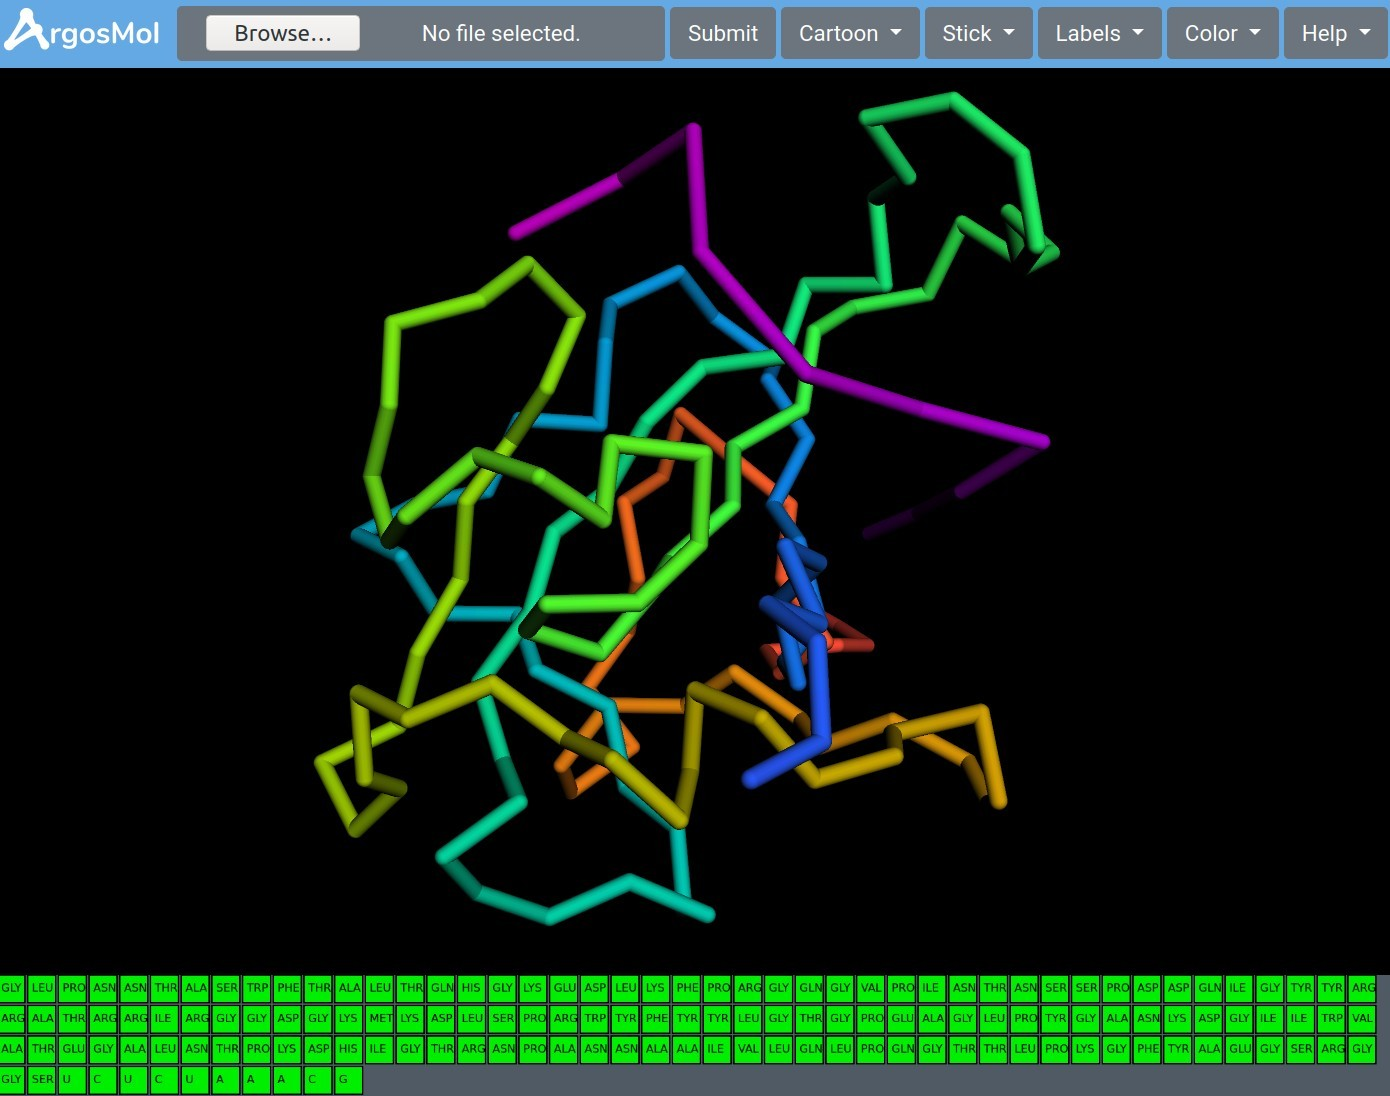
\includegraphics[width=.99\linewidth]{img/argosmol/mol3}
		\caption{}
		\label{fig:sfig2}
	\end{subfigure}
	\begin{subfigure}{.5\textwidth}
		\centering
		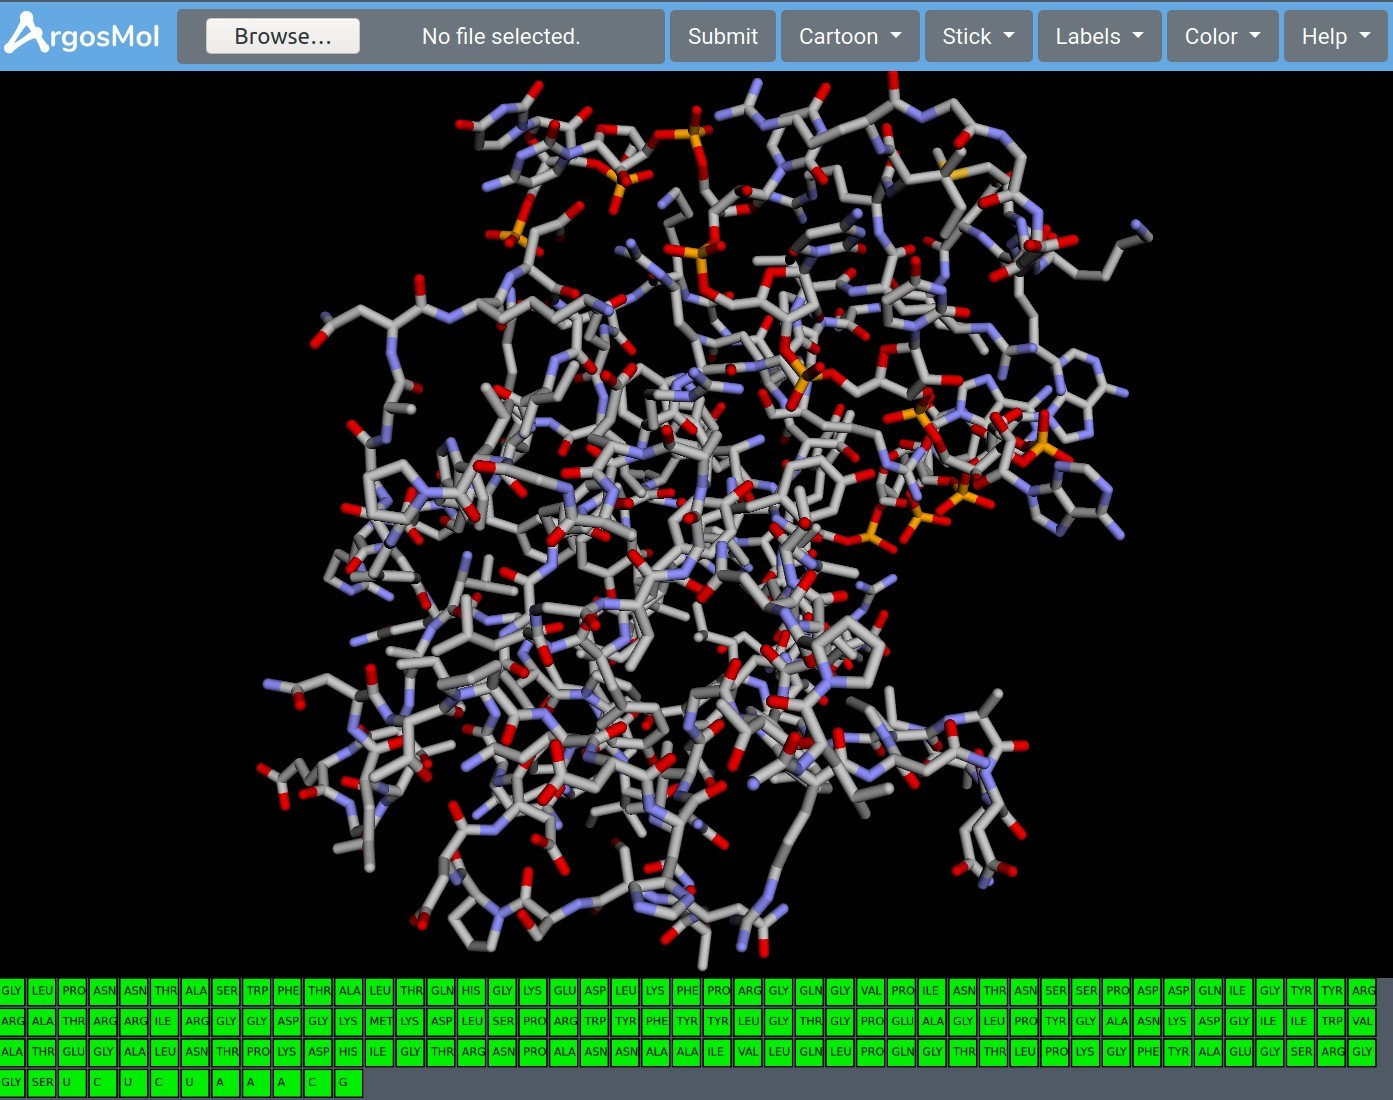
\includegraphics[width=.99\linewidth]{img/argosmol/mol4}
		\caption{}
		\label{fig:sfig1}
	\end{subfigure}%
	\begin{subfigure}{.5\textwidth}
		\centering
		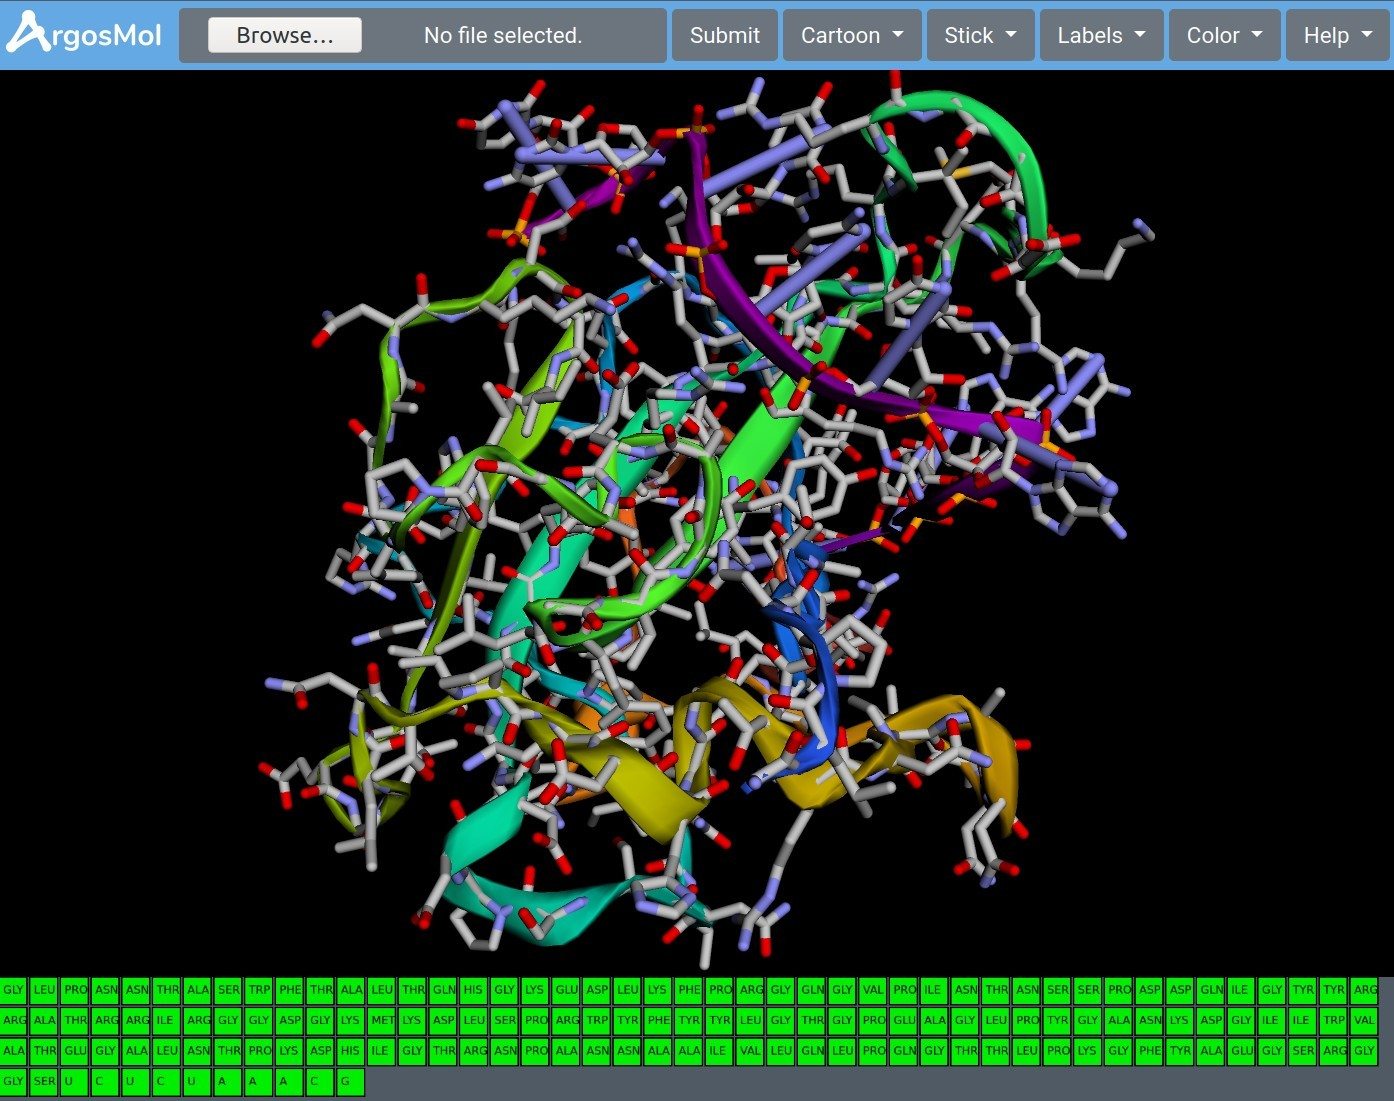
\includegraphics[width=.99\linewidth]{img/argosmol/mol5}
		\caption{}
		\label{fig:sfig2}
	\end{subfigure}
	\caption{Formas de visualizar una proteína en ArgosMol. (a) \textit{cartoon}, (b) \textit{trace}, (c) \textit{stick} y (d) \textit{cartoon}/\textit{stick}. }
	\label{fig:cartoon}
\end{figure}

\subsection{Esquema de colores}

ArgolMol tiene siete esquemas de colores, la vista por defecto es el color verde y se presenta en la Figura \ref{fig:argos1}. 
Los demas esquems de colors son descritos en la Tabla \ref{tab:color}

\begin{table}[h]

	\begin{tabular}{p{2.1cm} p{12.6cm}}
		\textbf{Esquema} & \textbf{Descripsión}   \\
		\hline 
		\textit{Spectrum} & Cada grupo de minoacidos es pintado aplicando una degradación de colores(Fig. \ref{fig:colors}.a). \\
		\textit{By chain} & Se asigna un color a cada cadena polipetídica (Fig. \ref{fig:colors}.b). \\
		\textit{By structure} & Se asigna un color según el tipo de estructura secundaria (Fig. \ref{fig:colors}.c). \\
		\textit{Rasmol color} & Se utiliza un color según la polaridad de cada aminoacido (Fig. \ref{fig:colors}.d). \\
		\textit{Rasmol shape} & Se utiliza un color según la forma de cada aminoacido (Fig. \ref{fig:colors}.e). \\
		\textit{MAE color} & Se utiliza el mismo esquema de colores que la herramienta MAE (Fig. \ref{fig:colors}.f). \\
		\hline
	\end{tabular}
\caption{Esquema de colores propuestos por ArgosMol.}
\label{tab:color}
\end{table}	

\begin{figure}[H]
	\begin{subfigure}{.5\textwidth}
		\centering
		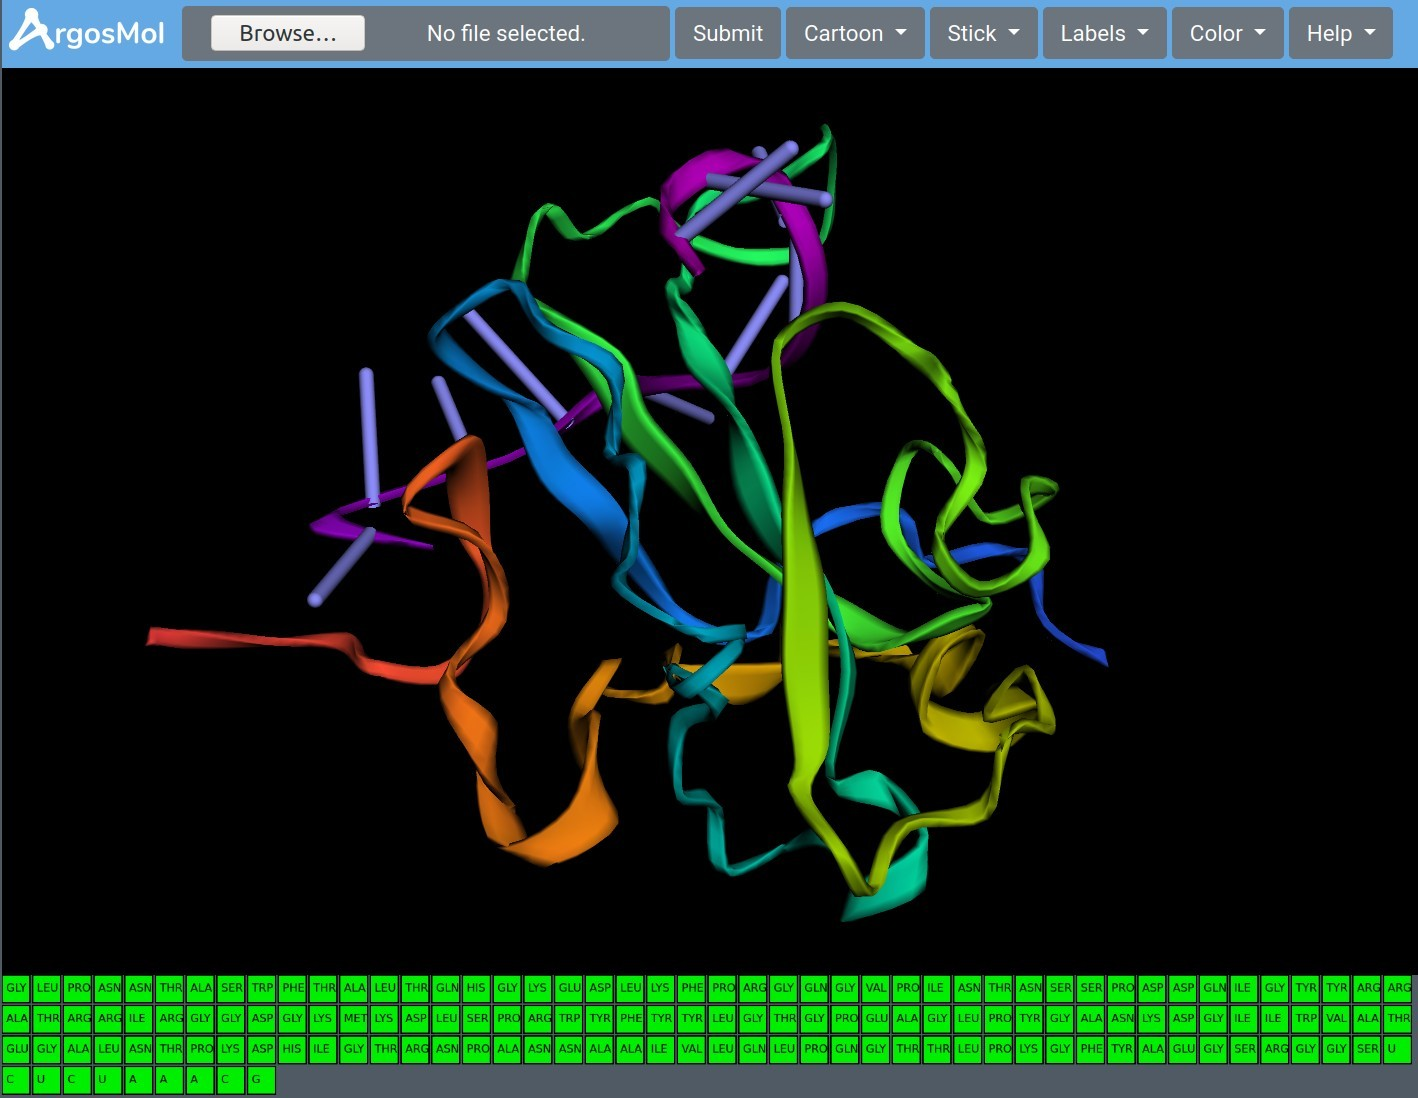
\includegraphics[width=.99\linewidth]{img/argosmol/mol6}
		\caption{}
		\label{fig:sfig1}
	\end{subfigure}%
	\begin{subfigure}{.5\textwidth}
		\centering
		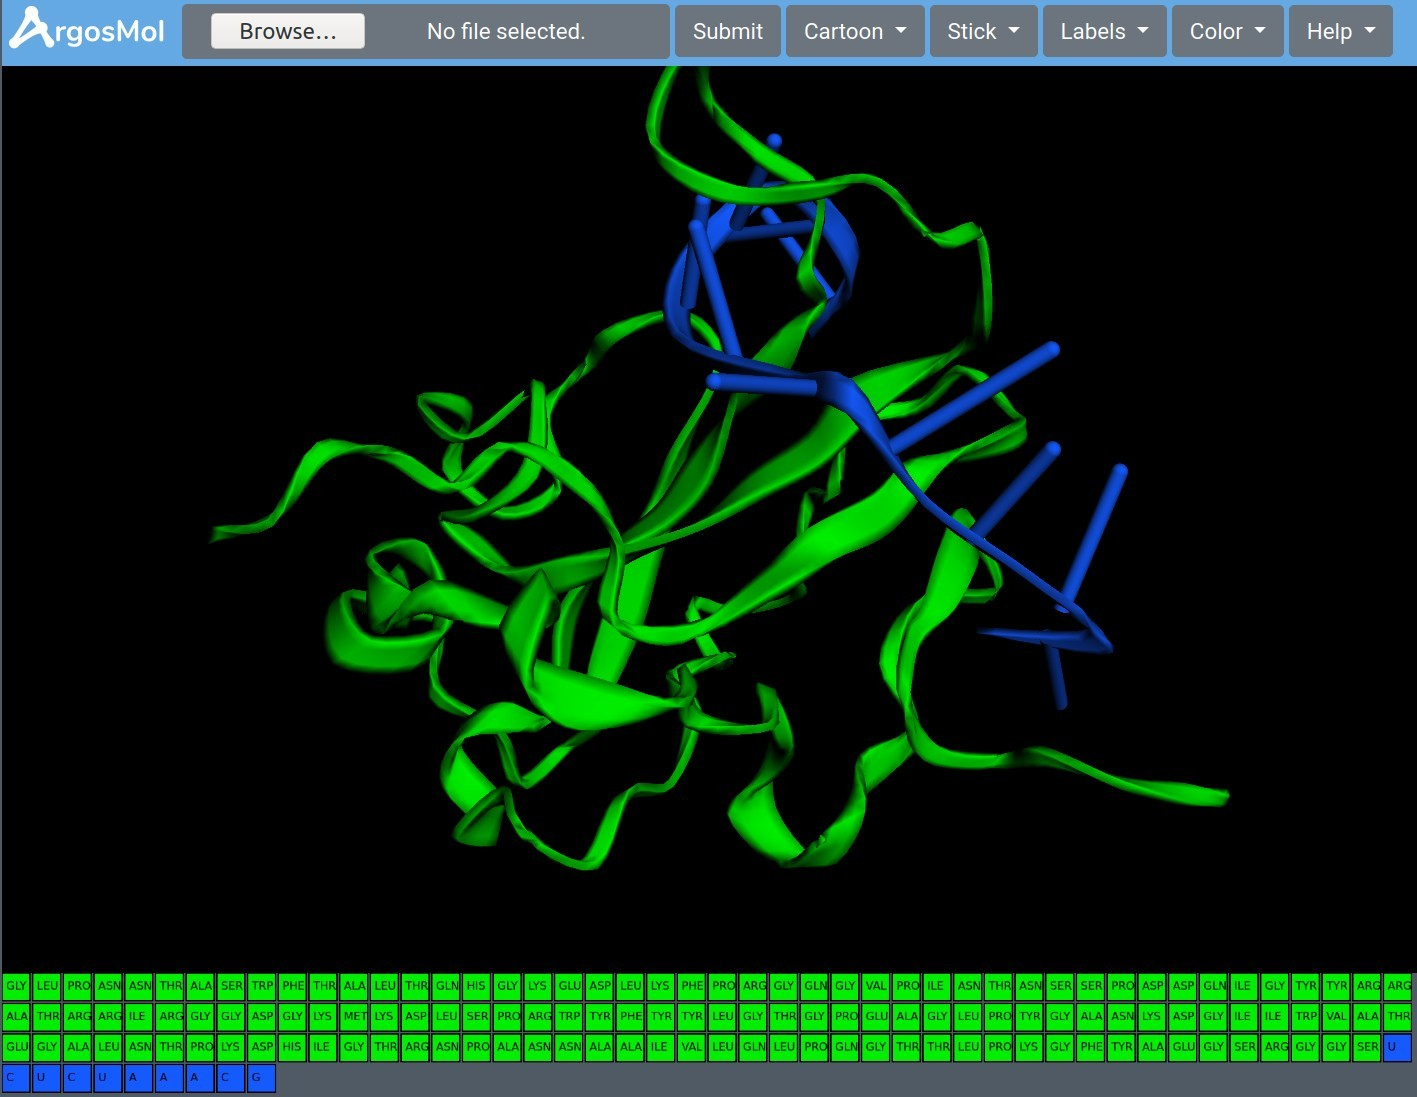
\includegraphics[width=.99\linewidth]{img/argosmol/mol7}
		\caption{}
		\label{fig:sfig2}
	\end{subfigure}
	\begin{subfigure}{.5\textwidth}
		\centering
		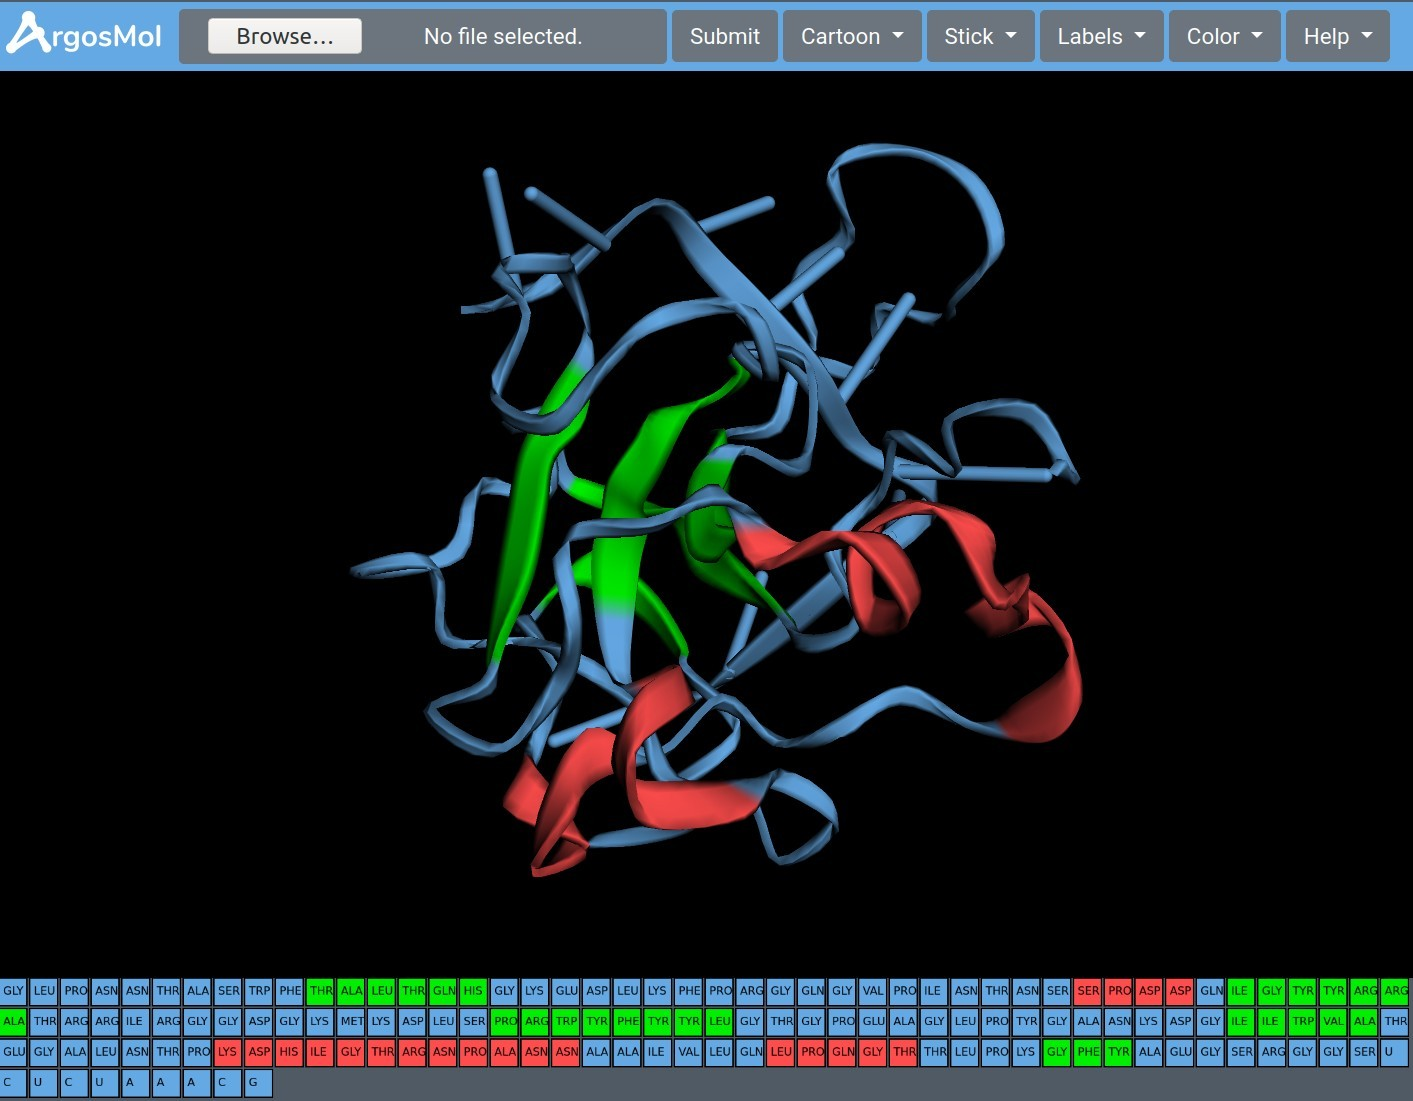
\includegraphics[width=.99\linewidth]{img/argosmol/mol8}
		\caption{}
		\label{fig:sfig1}
	\end{subfigure}%
	\begin{subfigure}{.5\textwidth}
		\centering
		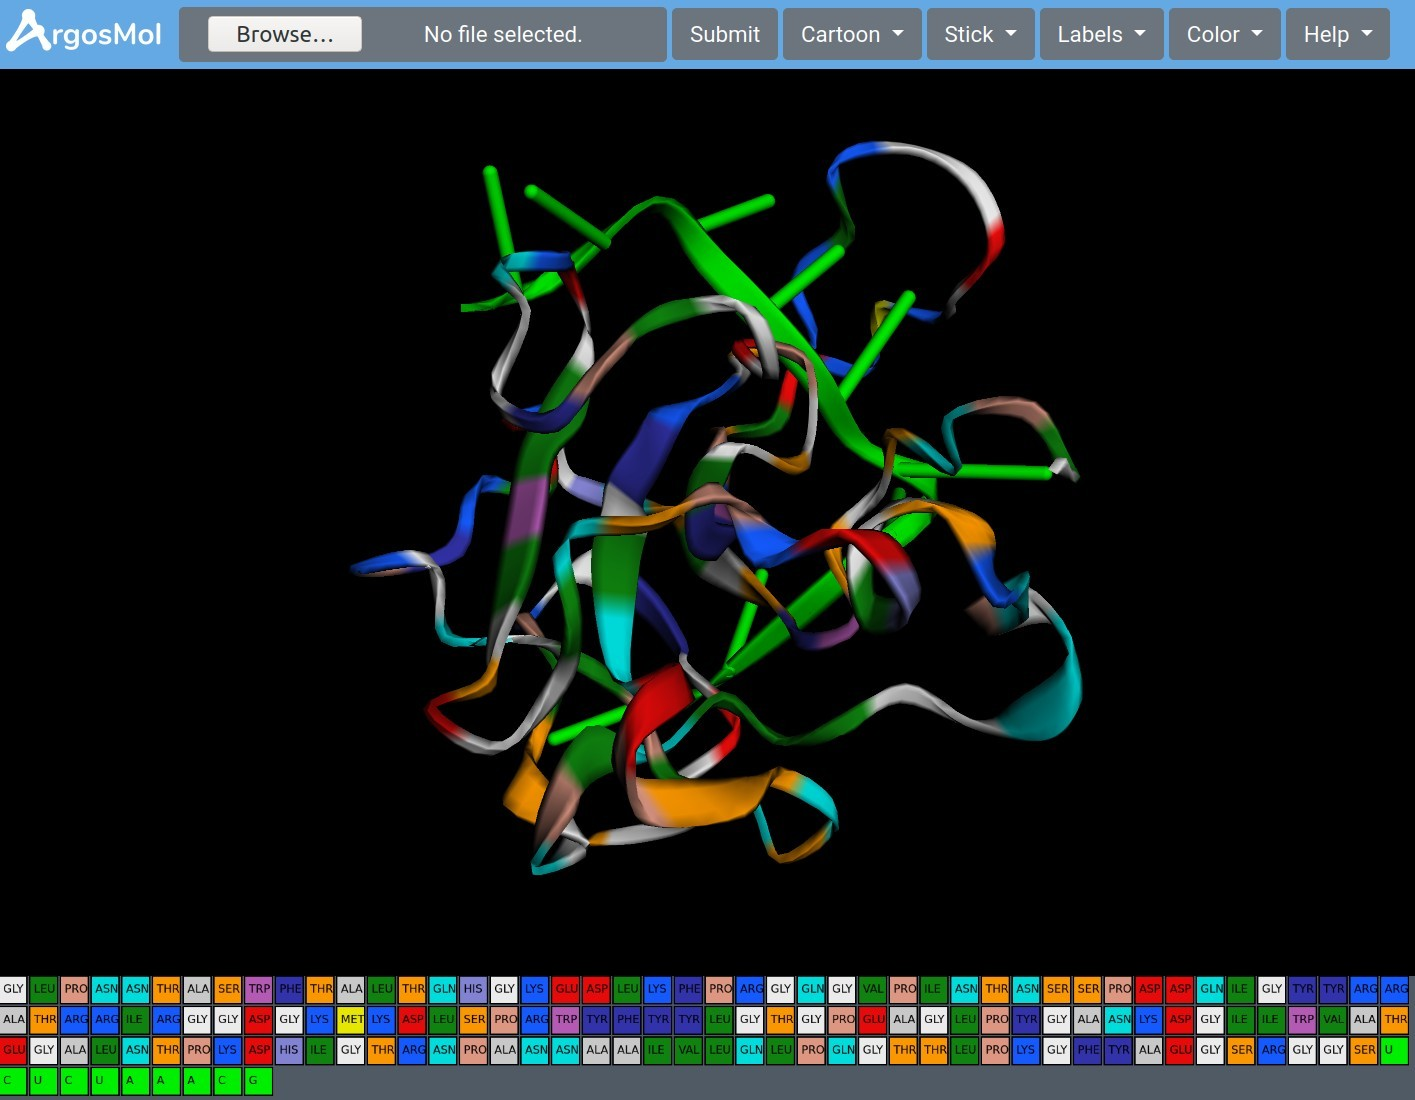
\includegraphics[width=.99\linewidth]{img/argosmol/mol9}
		\caption{}
		\label{fig:sfig2}
	\end{subfigure}
	\begin{subfigure}{.5\textwidth}
		\centering
		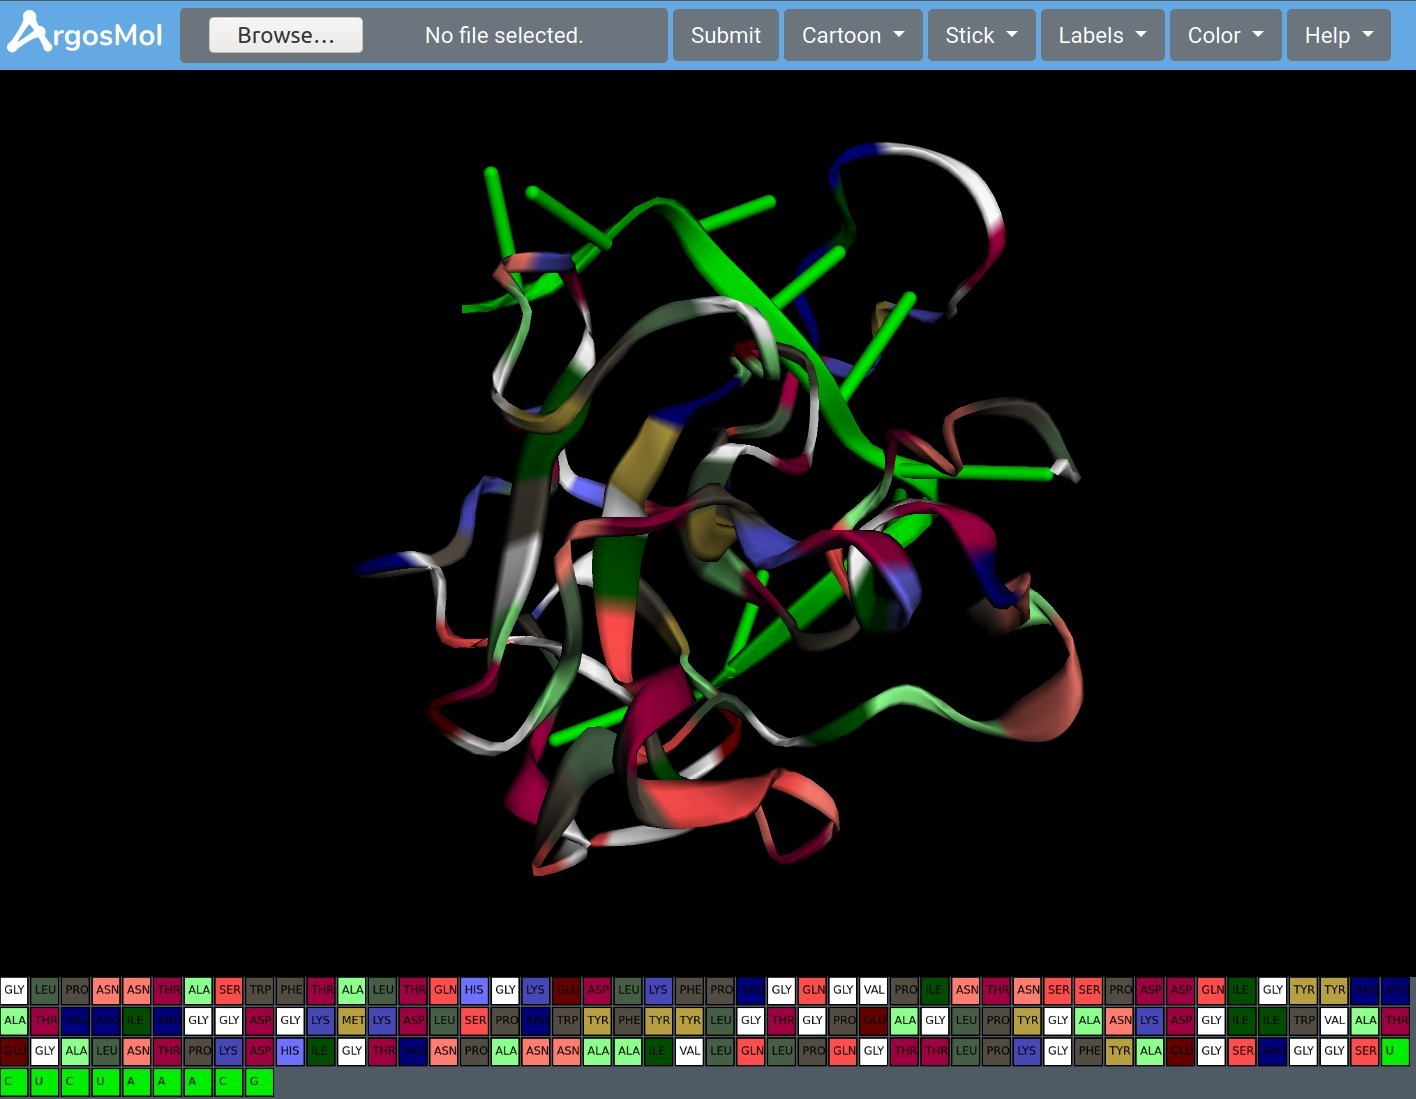
\includegraphics[width=.99\linewidth]{img/argosmol/mol10}
		\caption{}
		\label{fig:sfig1}
	\end{subfigure}%
	\begin{subfigure}{.5\textwidth}
		\centering
		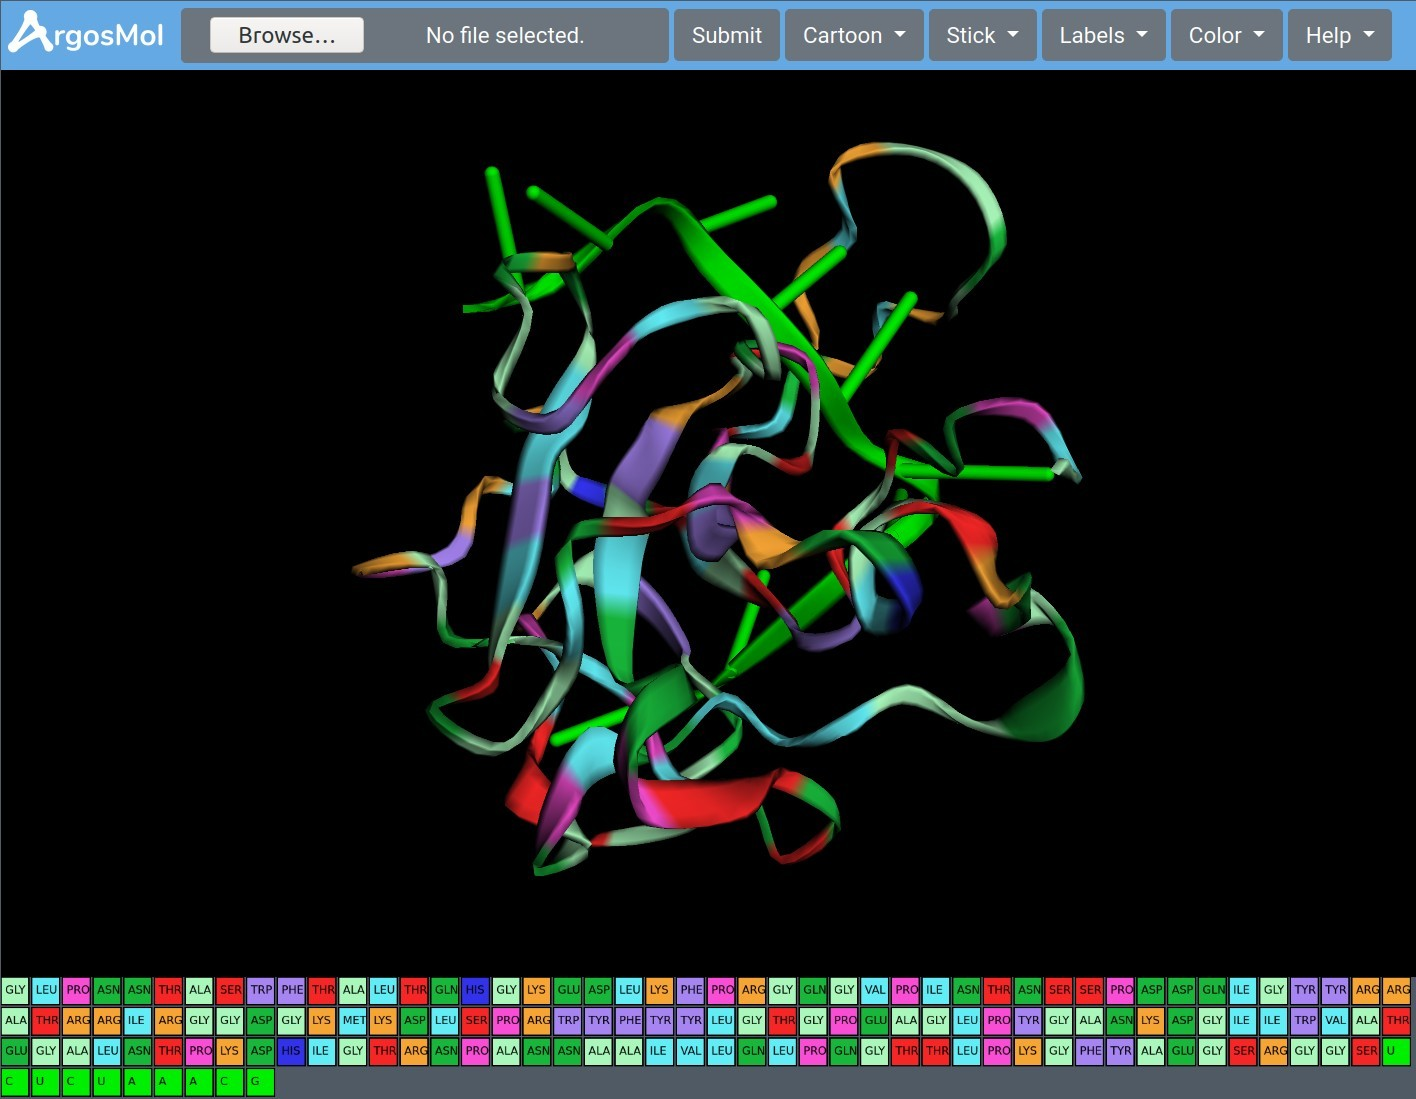
\includegraphics[width=.99\linewidth]{img/argosmol/mol11}
		\caption{}
		\label{fig:sfig2}
	\end{subfigure}
	\caption{Esquema de colores utilizados por ArgosMol ArgosMol. (a) \textit{spectrum}, (b) \textit{by chain}, (c) \textit{by structure} y (d) \textit{rasmol color}, (e) \textit{rasmol shape} y (f) \textit{MAE color}. }
	\label{fig:colors}
\end{figure}



\subsection{Secuencia de Aminoacidos}

\cite{youkharibache2017twelve} recomienda que toda herramienta de visualización debe incluir una vista a la secuencia de aminoacidos y estan deben estar enlazadas, de manera tal que si selecciono un aminoacido, este debe estar resaltado en el modelo. ArgosMol, ha tomado en cuenta esta requisito, por ejemplo en la Figura \ref{fig:clic}, mostramos como al hacer \textit{clic} izquierdo en algunos aminoacidos, estos son pintados de color verde tanto en el modelo; esta funcionalidad tambien puede ser utilizada de forma inversa, es decir: si hago \textit{clic} en el modelo, los aminoacidos en la secuencia serán resaltados.

\begin{figure}[H]
	\centering
	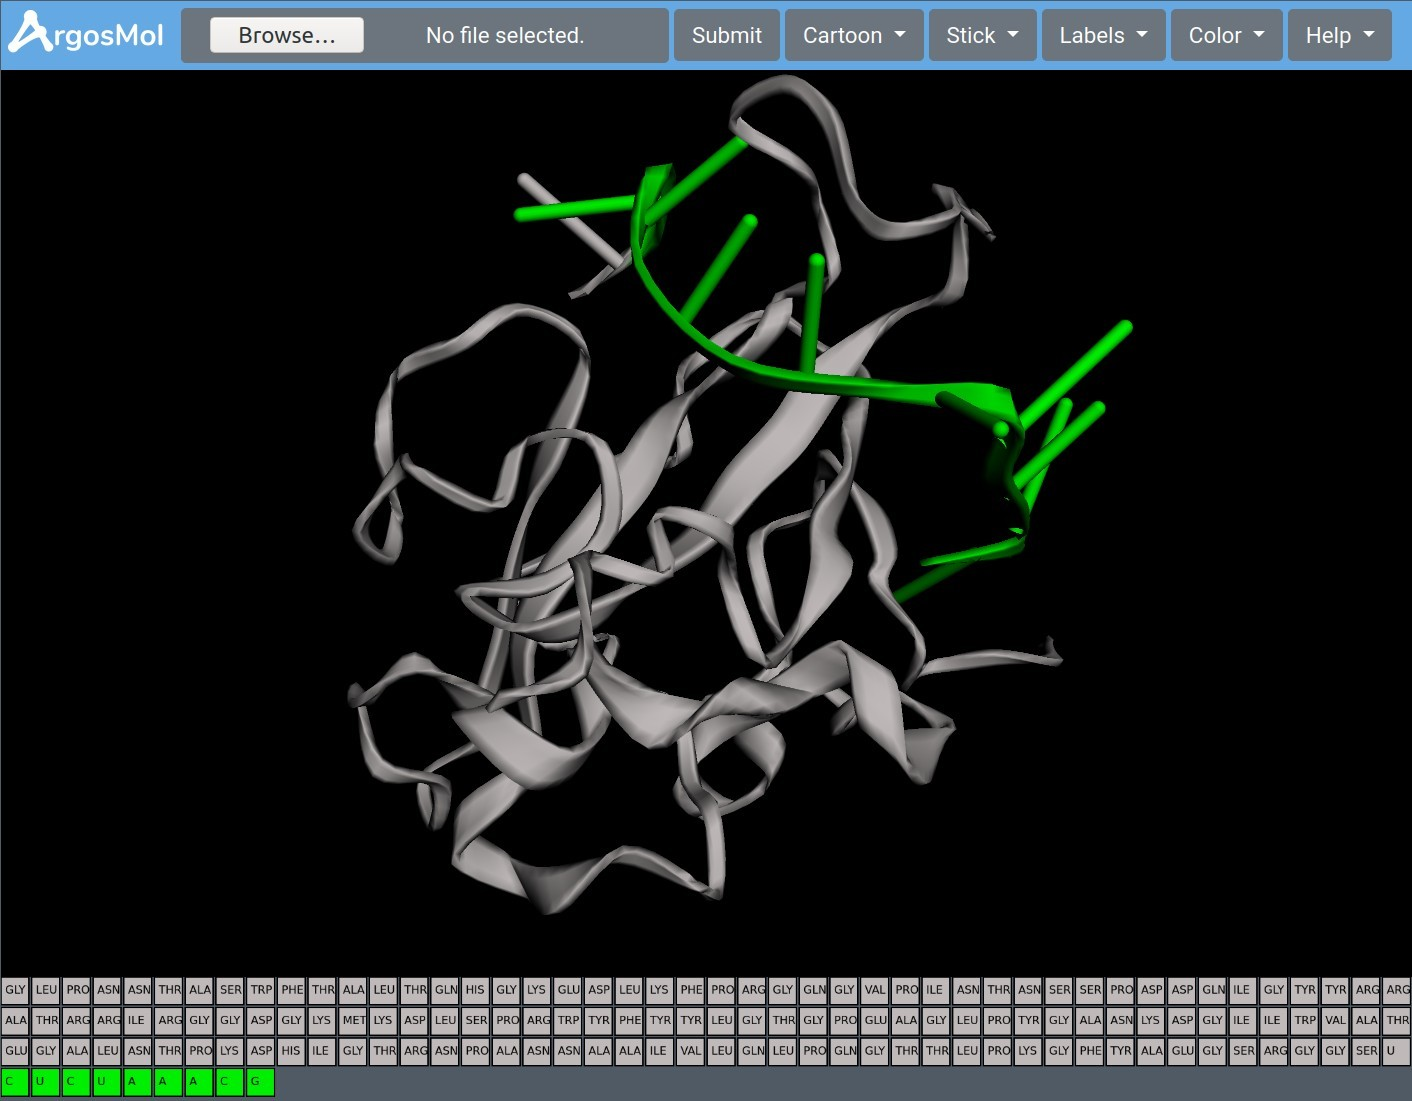
\includegraphics[width=\textwidth]{img/argosmol/mol12}
	\caption{ Ejemplo del enlace entre el modelo y la secuencia de aminoacidos mediante eventos del \textit{mouse}. }
	\label{fig:clic}
\end{figure}

\subsubsection{Eventos por teclado}

Tambien se ha agregado eventos por teclado para facilitar el uso de la herramienta, en la Tabla de tallamos estos eventos.

\begin{table}[H]
	
	\begin{tabular}{p{2.1cm} p{12.6cm}}
		\textbf{Teclado} & \textbf{Descripsión}   \\
		\hline 
		c & Activamos la opción para ver el \textit{cartoon}. \\
		C & Eliminamos el \textit{cartoon} del modelo. \\
		t & Activamos la opción para ver en estilo \textit{trace}. \\
		s & Activamos la opción para ver el \textit{stick}. \\ 
		S & Eliminamos el \textit{stick} del modelo. \\
		l & Agregamos todas las etiquetas de los aminoacidos al modelo. \\
		L & Eliminamos todas las etiquetas de los aminoacidos al modelo. \\
		r & Reiniciamos el modelo a su estado incial. \\
		Ctrl + z & Regresamoa a un estado anterior. \\
		\hline
	\end{tabular}
	\caption{Atajos de teclado utilizados en ArgosMol.}
	\label{tab:tecalado}
\end{table}	
	
\section{Trabajos futuros}
ArgosMol esta en su versión 1.0 permite ver la estructura terciaria de las proteínas, para versiones futuras se tiene planificado agregar la funcionalidad de ver las proteínas a nivel de moleculas. Tambien se tiene como objetivo a futuro, incorporar algoritmos de predicción de estructuras de proteínas, de manera tal, que tomando como entrada una secuencia de aminoacidos o un \textit{contact map}, ArgosMol genere la posición de cada atomo en un archivo .pdb.

\section{Conclusiones}

En este proyecto se ha estudiado el area de predicción de estructuras de proteínas y su visualización en herramientas Web. Al ser un trabajo complejo, se decidio enfocarnos en la visualización de proteínas y dejando la tarea de predicción de estructuras de proteínas como trabajo futuro.\\

Se propone la herramienta Web ArgosMol, la cual es una plataforma para la visualización de estructuras de proteínas, es de facil uso, y es una alternativa a herramientas de escritorio que requieren instalación y tienen una curva de aprendizaje alto.\\

Entre las funcionalidaddes de ArgosMol se propone 3 formas de visualización (\textit{cartoon, trace, stick}), varios esquemas de colores (por cadena polipeptídica, por tipo de estructura secundaria y según el tipo de aminoacido), atajos de teclado y un enlace permanente entre la secuencia de aminoacidos y el modelo 3D.
	
	\clearpage
	\bibliographystyle{apalike}
	%\bibliographystyle{IEEEtranN}
	\bibliography{bibliography}
	
	
	
	
	
\end{document}